\documentclass[review]{elsarticle}
\usepackage{comment}
\usepackage{url}
%
\usepackage[breaklinks]{hyperref}
\usepackage{breakurl}


\usepackage[ruled]{algorithm2e}

%\usepackage{lineno}
%\modulolinenumbers[5]

\journal{Optics Communications}

%%%%%%%%%%%%%%%%%%%%%%%
%% Elsevier bibliography styles
%%%%%%%%%%%%%%%%%%%%%%%
%% To change the style, put a % in front of the second line of the current style and
%% remove the % from the second line of the style you would like to use.
%%%%%%%%%%%%%%%%%%%%%%%

%% Numbered
%\bibliographystyle{model1-num-names}

%% Numbered without titles
%\bibliographystyle{model1a-num-names}

%% Harvard
%\bibliographystyle{model2-names.bst}\biboptions{authoryear}

%% Vancouver numbered
%\usepackage{numcompress}\bibliographystyle{model3-num-names}

%% Vancouver name/year
%\usepackage{numcompress}\bibliographystyle{model4-names}\biboptions{authoryear}

%% APA style
%\bibliographystyle{model5-names}\biboptions{authoryear}

%% AMA style
%\usepackage{numcompress}\bibliographystyle{model6-num-names}

%% `Elsevier LaTeX' style
\bibliographystyle{elsarticle-num}
%%%%%%%%%%%%%%%%%%%%%%%
\usepackage{graphicx}
\usepackage{subcaption}
%%%%%%%%%%%%%%%%%%%%%%%%%%%%%%%%%%%%%%%%%%%%%%%%%%%%%%%%%%%%%%%%%%%%%%%%%%%%%%%%%%

\usepackage[svgnames]{xcolor} % Enabling colors by their 'svgnames'

\usepackage{amsmath}
\usepackage{amsfonts}
\usepackage{amssymb}
%%%%%%%%%%%%%%%%%%%%%%%%%%%%%%%%%%%%%%%%%%%%%%%%%%%%%%%%%%%%%%%%%%%%%%%%%%%%%%%%%%

 
\begin{document} 

\begin{frontmatter}

\title{Importance of Sampling Frequency in the Dynamic Speckle Analysis}
%\tnotetext[mytitlenote]{Fully documented templates are available in the 
%elsarticle package on \href{http://www.ctan.org/tex-archive/macros/latex/contrib/elsarticle}{CTAN}.}



% Group authors per affiliation:
\author{------ ----- -----}
\author{------ ----- -----}



\address{University Federal of Lavras, Lavras, Brazil}
\fntext[myfootnote2]{201518201@posgrad.ufla.br}
\fntext[myfootnote1]{robertobraga@deg.ufla.br }
% 


\begin{abstract}
In this article, we show as the variation of sampling frequency, 
in a dynamic speckle analysis, affect the value of some dynamic speckle index, 
in this case: the absolute value of the differences index, the temporal 
speckle standard deviation index and the temporal 
speckle mean index.
we show that  the dynamic speckle index value decrease your maximum excursion with 
the grow of sampling frequency because this affect directly the time integration 
(exposition time) of camera.
\end{abstract}

\begin{keyword}
Frequency sampling \sep
Dynamic speckle index \sep 
Dynamic speckle index \sep 
Dynamic speckle analysis
\end{keyword}

\end{frontmatter}

\linenumbers


%%%%%%%%%%%%%%%%%%%%%%%%%%%%%%%%%%%%%%%%%%%%%%%%%%%%%%%%%%%%%%%%%%%%%%%%%%%%%%%%
%%%%%%%%%%%%%%%%%%%%%%%%%%%%%%%%%%%%%%%%%%%%%%%%%%%%%%%%%%%%%%%%%%%%%%%%%%%%%%%%
%%%%%%%%%%%%%%%%%%%%%%%%%%%%%%%%%%%%%%%%%%%%%%%%%%%%%%%%%%%%%%%%%%%%%%%%%%%%%%%%
%%%%%%%%%%%%%%%%%%%%%%%%%%%%%%%%%%%%%%%%%%%%%%%%%%%%%%%%%%%%%%%%%%%%%%%%%%%%%%%%
\section{Introduction}


%1) Anuncie o tema e o problema do artigo (forma de pergunta + definiçoes)




The dynamic laser speckle analysis has become in the last years  an important
study topic\cite{catalano2019viability,rivera2019sound,gonzalez2018diode,Silva2018,braga2017dynamic} 
to determine the  activity level of biological materials. 
The importance of technical aspects of dynamic laser speckle analysis,
as the stability of laser illumination level has been  analyzed \cite{gonzalez2018diode}; 
and also It was studed as indexes,
as absolute values of the differences \cite{cardoso2014,rivera2017selection} are affected in your values
by the variation of illumination level. Thus, It is necessary analyze the effect
of technical parameters that affect the perceived illumination level; In these sense
we analyze the effect of sampling frequency in a dynamic laser speckle analysis. 




%2) Exponha qual será o percurso (defina seçoes)
%3) Resgate a problematica( Importancia do problema de pesquisa - extenda primer passo)
%4) Relevancia do artigo(importancia para outros del artigo publicado)
%5) Anuncie a hipotesi
%6) Anuncie os objetivos (receita pra demostrar a h.)

%%%%%%%%%%%%%%%%%%%%%%%%%%%%%%%%%%%%%%%%%%%%%%%%%%%%%%%%%%%%%%%%%%%%%%%%%%%%%%%%
%%%%%%%%%%%%%%%%%%%%%%%%%%%%%%%%%%%%%%%%%%%%%%%%%%%%%%%%%%%%%%%%%%%%%%%%%%%%%%%%
%%%%%%%%%%%%%%%%%%%%%%%%%%%%%%%%%%%%%%%%%%%%%%%%%%%%%%%%%%%%%%%%%%%%%%%%%%%%%%%%
%%%%%%%%%%%%%%%%%%%%%%%%%%%%%%%%%%%%%%%%%%%%%%%%%%%%%%%%%%%%%%%%%%%%%%%%%%%%%%%%
\section{System description}
\label{sec:description}




\subsection{Exposure time of the camera}
\label{subsec:expositiontime}
The acquisition time,  frame per seconds ($fps$) or sampling frequency ($F_s$), 
in the camera Marlin F-033 will be calculated in the 
 Table \ref{table:1}, where we can see, the shutter register value ($Shutter$), 
time base register value ($Base$),
exposure time ($Exposure$),
exposure time offset ($Offset$) and
effective exposure time ($E$); so that 
\begin{equation}
Exposure= Shutter \times Base,
\end{equation}
\begin{equation}
\frac{1}{F_s}=E= Exposure + Offset.
\end{equation}
Where,  $F_s$ is calculated in relation to the  $E$; being that,
the $Exposure$ represent the photography integration time and $E$ the effective time
between photographs; 
the difference between these two exposures arise from $Offset$ time, 
that is the time between end and start of a photography.
\begin{table}[h!]
\centering
\begin{tabular}{||c c c c c||} 
 \hline
 $Shutter$ &  $Base$ [$\mu s$] & $Offset$ [$\mu s$] & $E$ [$ms$] & $F_s$ [$fps$]\\ [0.5ex] 
 \hline\hline
 3332  & 20  & 12  & 66.652  & 15.003  \\ 
 1665  & 20  & 12  & 33.312  & 30.019  \\ 
 1110  & 20  & 12  & 22.212  & 45.021  \\ 
 832   & 20  & 12  & 16.652  & 60.053  \\ [1ex] 
 \hline
\end{tabular}
\caption{Exposition time and sampling frequency}
\label{table:1}
\end{table}

\subsection{Data packages in the ink drying process}
\label{subsec:data1}
 This data package analyze a drying ink process, 
 where images data packages are taken at the times
 $\{0,$ $1,$ $2,$ $3,$ $4,$ $5,$ $6,$ $7,$ $8,$ $9,$ $10\}$ min. 
 In each time, the package
 has 512 images of 147 pixels of height and 166 pixels of width.
 They were use 4 different sampling frequencies to the images in each package,
 being these frequencies $15$, $30$, $45$ and $60$ hz.

\subsection{Data package of the activity analysis in corn seed}
\label{subsec:data2}
 This data package analyze the activity of a corn seed with 3 days of germination. 
 In this point, 
 They are taken 4 image data packages with different sampling frequencies to each package,
 being these frequencies $15$, $30$, $45$ and $60$ hz.
 Each package has 512 images of $15$ pixels of height and $15$ pixels of width.
 

\subsection{Test 1: ink drying process}
\label{subsec:test1}
The Fig. \ref{fig:test1} represents the data analysis method, acquired at a 
sampling frequency of $F_s$, 
with the characteristic seen in the Section \ref{subsec:data1},
\begin{figure}[ht!]
\centering
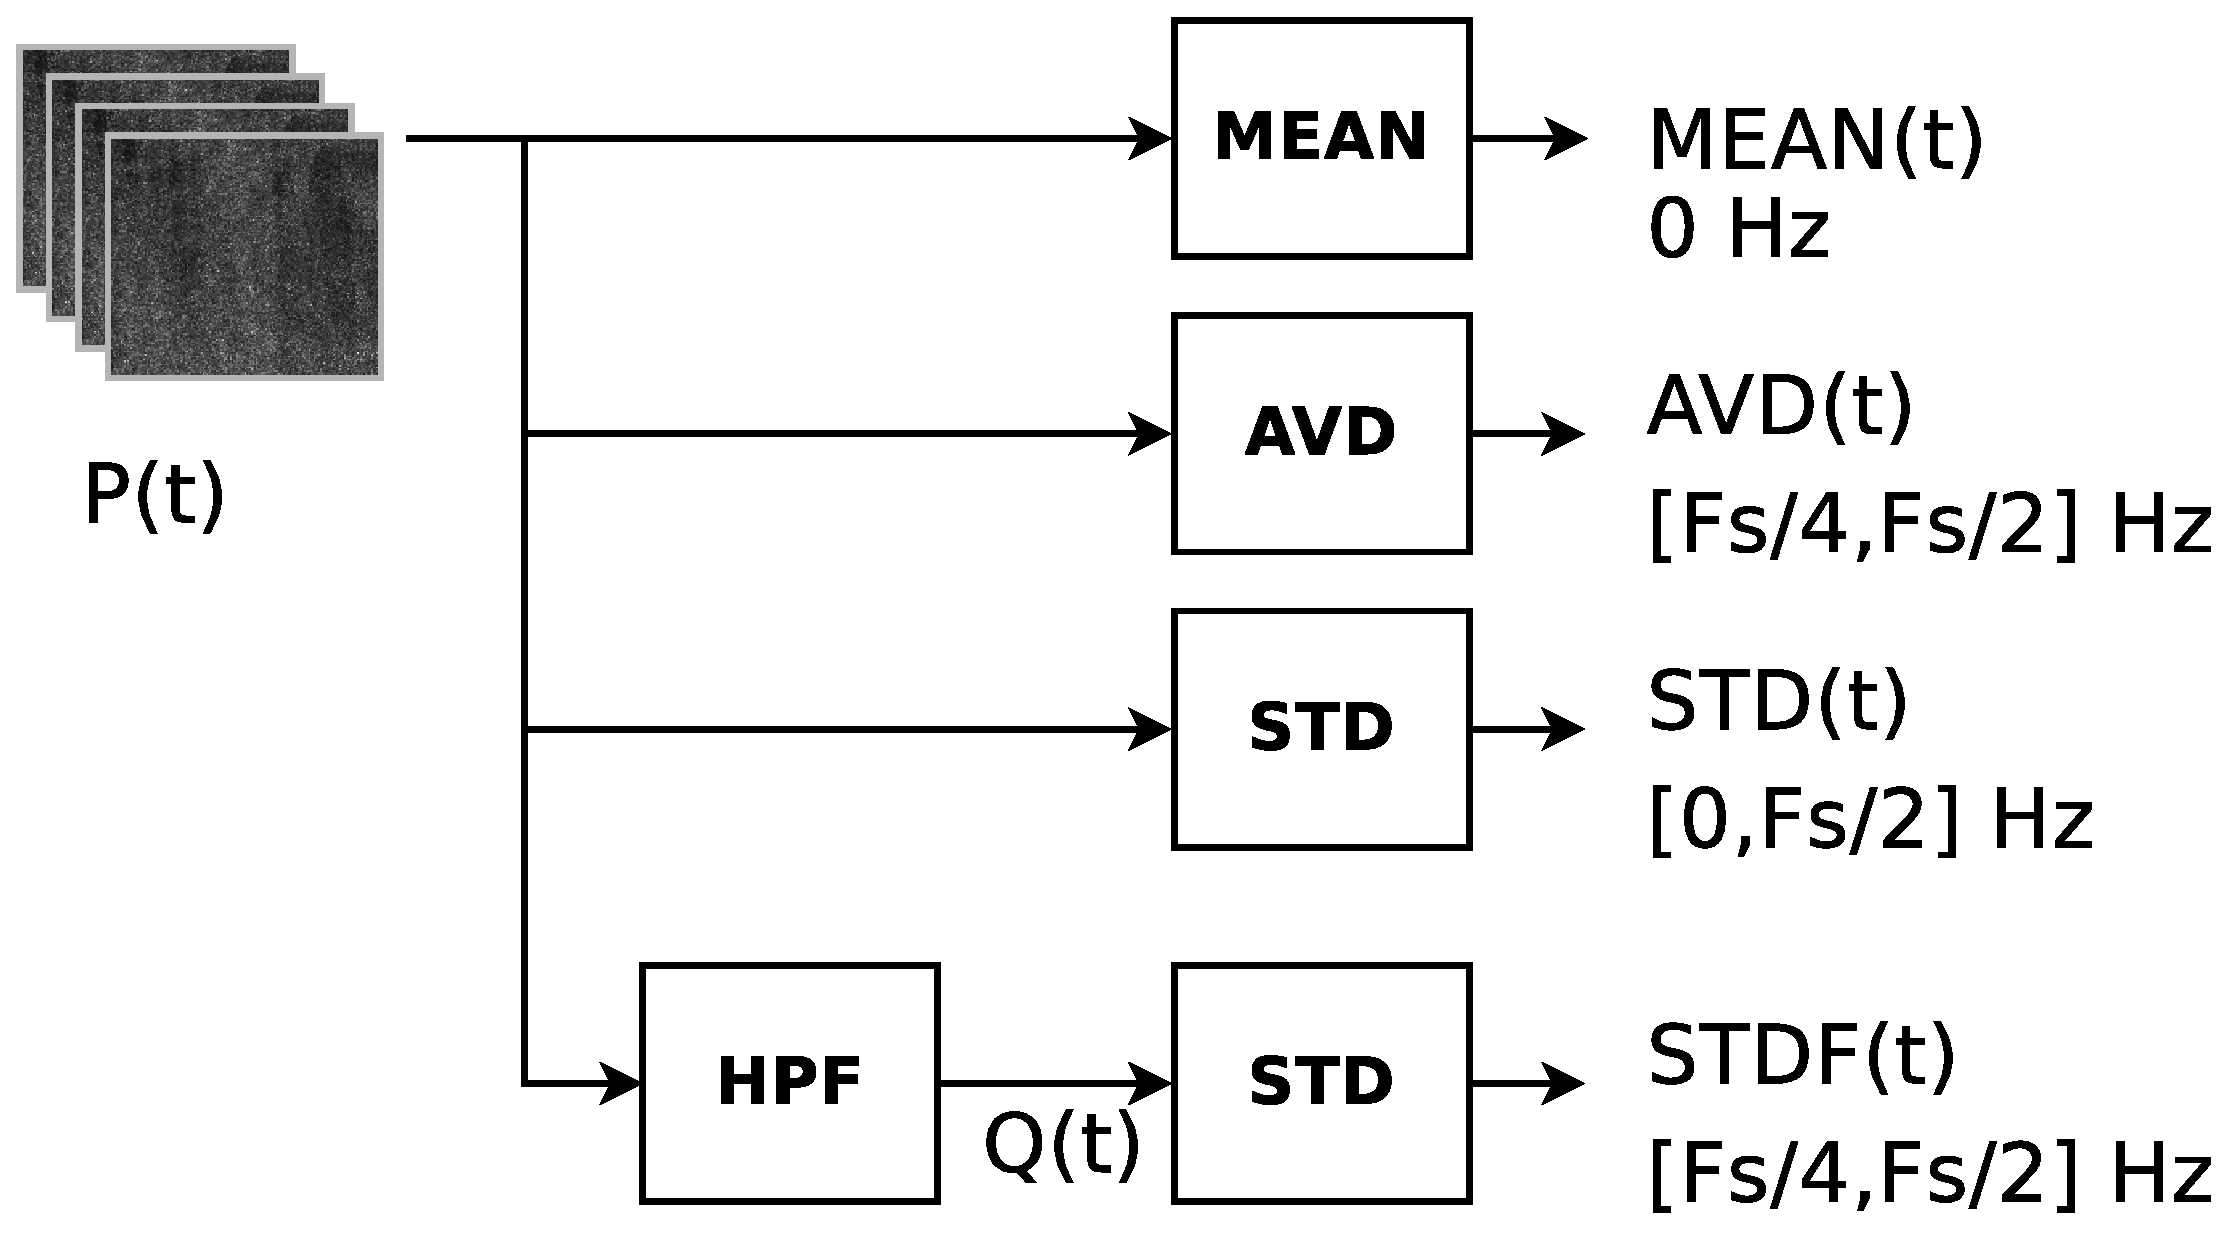
\includegraphics[width=0.55\columnwidth]{test1.eps}
\caption{Data analysis of the ink drying process test.}
\label{fig:test1}
\end{figure}
where, $P(t)$ is an image data package at the time $t$ minutes, 
being that this package has $N$ images and $M$ pixels, where $P_{n,m}(t)$ 
define the $n$-th image and $m$-th pixel, for all $1 \leq n \leq N$, $1 \leq m \leq M$.
The $MEAN$ block represents the calculus of a temporal speckle mean index from 
the package $P(t)$, returning the value $MEAN(t)$, as exposed in the Section \ref{sec:mean}. 
The $AVD$ block represents the calculus of an absolute values of the differences index from 
the package $P(t)$, returning the value $AVD(t)$, as exposed in the Section \ref{sec:avd}. 
The $STD$ block represents the calculus of a temporal speckle standard deviation index from 
the package $P(t)$, returning the value $STD(t)$, as exposed in the Section \ref{sec:std}.
And finally,
the block $HPF$ represents a digital finite impulse response ``high-pass filter'' 
with order $40$ and cut-off at $0.25F_s$ and this block filter the $P(t)$ package and return $Q(t)$,
that causes to have at end of path the $STDF(t)$ index value.
According the information of the data packages, 
we will have speckle indexes values, for each minute during 10 minutes.

\subsection{Test 2: Activity analysis in corn seed}
\label{subsec:test2}
The activity analysis of a corn seed, 
uses the information of data package seen in the Section \ref{subsec:data2}.
We analyze this information of similar way to the seen in the Section \ref{subsec:test1},
with the difference that is taken an data package at the time $t$ (3 days of germination)
and a sampling frequency $F_s$. 

\subsection{Test 3: Frequency band activity analysis}
\label{subsec:test3}

The Fig. \ref{fig:test3} represents the frequency band analysis method of data package $P$, 
acquired  with a sampling frequency of $F_s$. This package pass through the $BPF$ block
described in the Sec \ref{sec:stdb}, with a frequency band pass between $f_1(l)$ and $f_2(l)$,
according the Eq. \ref{eq:f1f2}, where $l$ represent the band so that $1\leq l\leq L$,
being $L$ the quantity of analysis frequency bands; 
thus, we obtaining the  $R$ package (a filtered version of $P$). Later, It is processed 
a $\sigma$ block, where It is calculate the $\sigma_{m}$ value to each pixel in the package $R$,
as described in the Sec \ref{sec:std}. Finally, 
an image is obtained and It is designed with the variable $STDB$.
\begin{figure}[ht!]
\centering
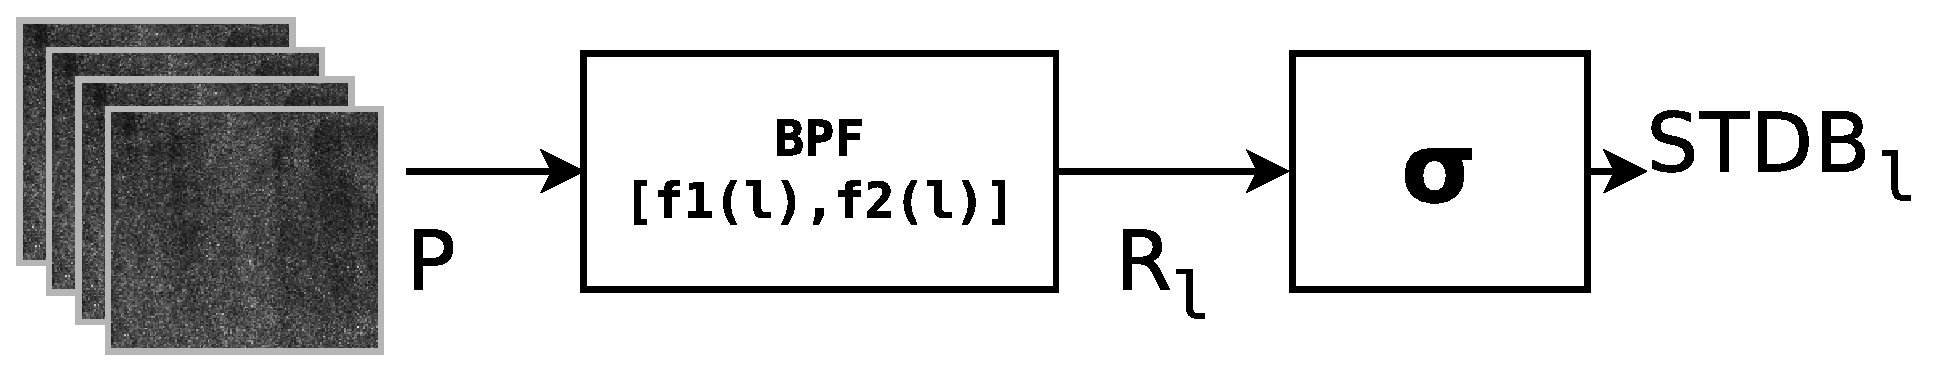
\includegraphics[width=0.55\columnwidth]{test3.eps}
\caption{Frequency band analysis of a data package.}
\label{fig:test3}
\end{figure}

 

%%%%%%%%%%%%%%%%%%%%%%%%%%%%%%%%%%%%%%%%%%%%%%%%%%%%%%%%%%%%%%%%%%%%%%%%%%%%%%%%
%%%%%%%%%%%%%%%%%%%%%%%%%%%%%%%%%%%%%%%%%%%%%%%%%%%%%%%%%%%%%%%%%%%%%%%%%%%%%%%%
%%%%%%%%%%%%%%%%%%%%%%%%%%%%%%%%%%%%%%%%%%%%%%%%%%%%%%%%%%%%%%%%%%%%%%%%%%%%%%%%
%%%%%%%%%%%%%%%%%%%%%%%%%%%%%%%%%%%%%%%%%%%%%%%%%%%%%%%%%%%%%%%%%%%%%%%%%%%%%%%%
\section{Theoretical definitions}
\label{sec:theoretical}

In the next subsections we use the variable $P$ to define $P(t)$ in any time $t$.

\subsection{$MEAN$ index }
\label{sec:mean}

The temporal speckle mean index ($\mu_{m}$) \cite{Nothdurft:05} calculates the mean
value of the illumination level to the $m$-th pixel in the package $P$, It is implemented
with the Eq. \ref{eq:mu},
\begin{equation}\label{eq:mu}
\mu_{m} = \sum \limits_{n=1}^{N} \frac{P_{n,m}}{N}.
\end{equation}
Finally, the $MEAN$ index is the mean value of all $\mu_{m}$ results,
as can be viewed in the Eq. \ref{eq:MEAN},
\begin{equation}\label{eq:MEAN}
MEAN = \sum \limits_{m=1}^{M} \frac{\mu_{m}}{M}.
\end{equation}


\subsection{$AVD$ index}
\label{sec:avd}

The Absolute Values of the Differences ($AVD_{m}$) \cite{cardoso2014,rivera2017selection} calculates the mean
value of the absolute differences in the illumination level of the $m$-th pixel in the package $P$, It is implemented
with the Eq. \ref{eq:avd0},
\begin{equation}\label{eq:avd0}
AVD_{m} = \sum \limits_{n=2}^{N} \frac{|P_{n,m}-P_{n-1,m}|}{N}.
\end{equation}
Finally, the $AVD$ index is the mean value of all $AVD_{m}$ results,
as can be viewed in the Eq. \ref{eq:AVD},
\begin{equation}\label{eq:AVD}
AVD = \sum \limits_{m=1}^{M} \frac{AVD_{m}}{M}
\end{equation}

%Frequency composition from $F_s/4$ until $F_s/2$ Hz like as  $HPF$ of first order.


\subsection{$STD$ index}
\label{sec:std}


The temporal speckle standard deviation index ($\sigma_{m}$) \cite{Nothdurft:05} calculates the standard deviation
value of the illumination level to the $m$-th pixel in the package $P$, It is implemented
with the Eq. \ref{eq:sigma},
\begin{equation}\label{eq:sigma}
\sigma_{m}^2 = \sum \limits_{n=1}^{N} \frac{(P_{n,m}-\mu_{m})^2}{N}.
\end{equation}
Finally, the $STD$ index is the mean value of all $\sigma_{m}$ results,
as can be viewed in the Eq. \ref{eq:STD},
\begin{equation}\label{eq:STD}
STD = \sum \limits_{m=1}^{M} \frac{\sigma_{m}}{M}
\end{equation}

%Frequency composition from $0$ until $F_s/2$ Hz like as  $HPF$ of first order.

\subsection{$HPF$ block}
\label{sec:stdf}

The high-pass filter ($HPF$) block It is implemented with a finite impulse 
response ($FIR$)\cite{saramaki1993finite} filter
of order 40 and cut-off at $0.25F_s$. 
The 41 values in the filter are represented with $h(i)$, for all $0 \leq i\leq 40$ and zero in others cases, so that
if we send a data package $P$ through the $HPF$ block we obtain a data package $Q$,
as can be seen in the Eq. \ref{eq:fir},
\begin{equation}\label{eq:fir}
Q_{n,m} = \sum_{k=1}^{N} P_{k,m} h(n-k+20}).
\end{equation}

%Frequency composition from $0$ until $F_s/2$ Hz like as  $HPF$ of first order.

\subsection{$BPF$ block}
\label{sec:stdb}

The band-pass filter ($BPF$) block, 
It is implemented similarly as the see in Sec. \ref{sec:stdf}, 
 with  a $FIR$ filter of order 40 but with a cut-off in $f_1(l)$ and $f_2(l)$, 
\begin{equation}\label{eq:f1f2}
\left [ f_1(l),~f_2(l)\right ] = \left [\frac{(l-1)}{L},~\frac{l}{L} \right ]\frac{F_s}{2},
\end{equation}
representing $l$, for all $1 \leq l \leq L$, the $l$-th band of $L$ parts; so that each band has $\frac{F_s}{2L}$ Hz.
The filter is represented with $g(i)$, for all $0 \leq i\leq 40$ and zero in others cases, so that
if we send a data package $P$ through the $BPF$ block we obtain a data package $R$,
as can be seen in the Eq. \ref{eq:firb},
\begin{equation}\label{eq:firb}
R_{n,m} = \sum_{k=1}^{N} P_{k,m}~g(n-k+20}).
\end{equation}

%%%%%%%%%%%%%%%%%%%%%%%%%%%%%%%%%%%%%%%%%%%%%%%%%%%%%%%%%%%%%%%%%%%%%%%%%%%%%%%%
%%%%%%%%%%%%%%%%%%%%%%%%%%%%%%%%%%%%%%%%%%%%%%%%%%%%%%%%%%%%%%%%%%%%%%%%%%%%%%%%
%%%%%%%%%%%%%%%%%%%%%%%%%%%%%%%%%%%%%%%%%%%%%%%%%%%%%%%%%%%%%%%%%%%%%%%%%%%%%%%%
%%%%%%%%%%%%%%%%%%%%%%%%%%%%%%%%%%%%%%%%%%%%%%%%%%%%%%%%%%%%%%%%%%%%%%%%%%%%%%%%
\section{Numerical results} 
\label{sec:numericalresults}

%%%%%%%%%%%%%%%%%%%%%%%%%%%%%%%%%%%%%%%%%%%%%%%%%%%%%%%%%%%%%%%%%%%%%%%%%%%%%%%%
\subsection{Result of test 1}
\label{subsec:resulttest1}
This test shows the analyze result of an ink drying process, across 10 minutes,
with the sampling frequency: $15$, $30$, $45$ and $60$Hz.

%%%%%%%%%%%%%%%%%%%%%%%%%%%%%%%%%%%%%%%%%%%%%%%%%%%%%%%%%%%%%%%%%%%%%%%%%%%%%%%%
The Figure \ref{fig:MEANtest1} analyze the $MEAN(t)$ index,
in the test showed in the Section \ref{subsec:test1},
to each time $t$ for 4 sampling frequencies.
\begin{figure}[ht!]
    \centering
    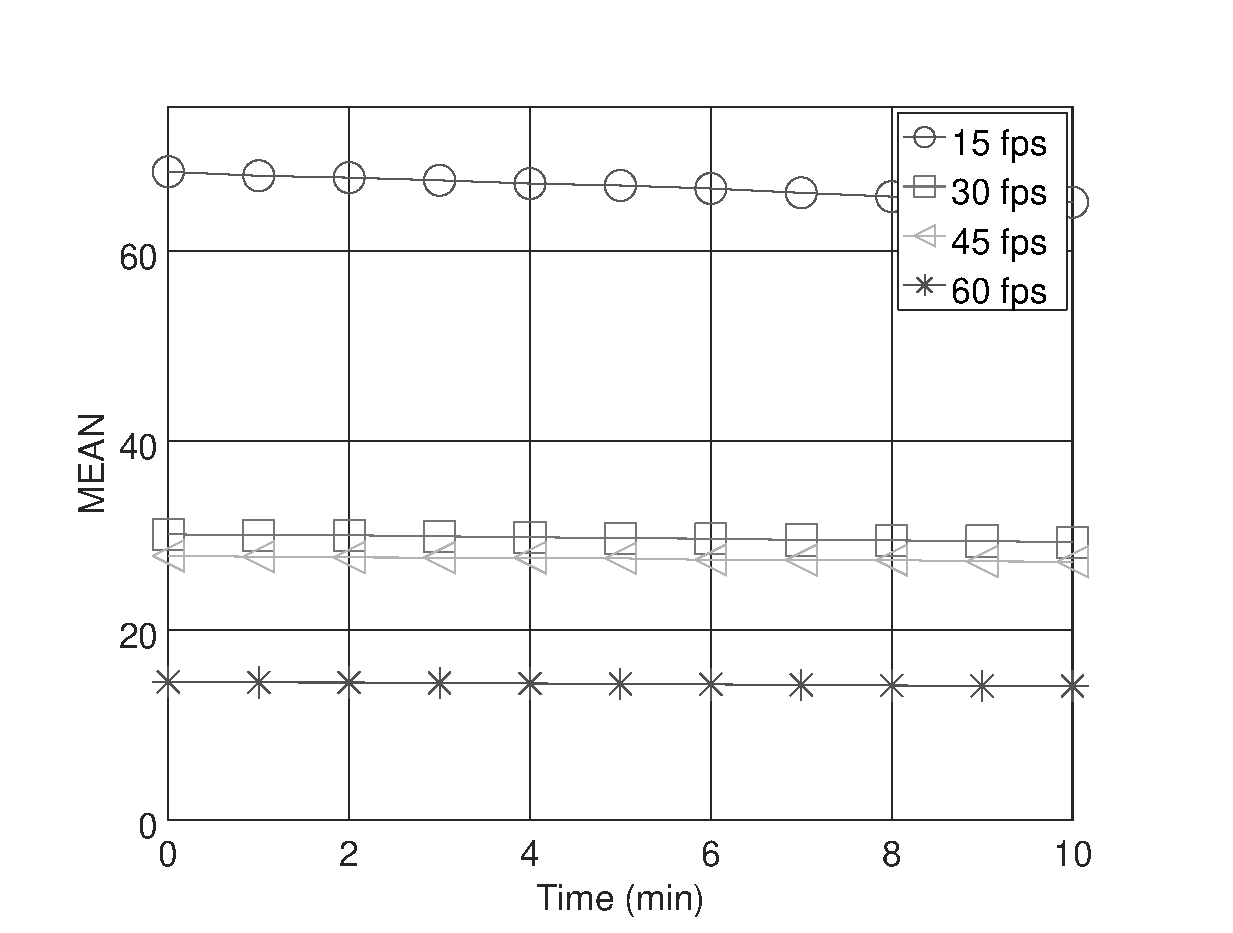
\includegraphics[width=0.5\textwidth]{FPS_f11_rawMEAN.eps}
    \caption{$MEAN$ index value.}\label{fig:MEANtest1}
\end{figure}
It easy to see as the value of index has a monotonous 
behavior over time. By other side the values in the curves decreases in proportion with 
the grow of sampling frequency.

%%%%%%%%%%%%%%%%%%%%%%%%%%%%%%%%%%%%%%%%%%%%%%%%%%%%%%%%%%%%%%%%%%%%%%%%%%%%%%%%
The Figure \ref{fig:AVDtest1} shows the result of analysis explained in the 
Section \ref{subsec:test1} about the $AVD(t)$ index.
\begin{figure}[ht!]
    \centering
    \begin{subfigure}{0.48\textwidth}
        \caption{$AVD$ index value.}
        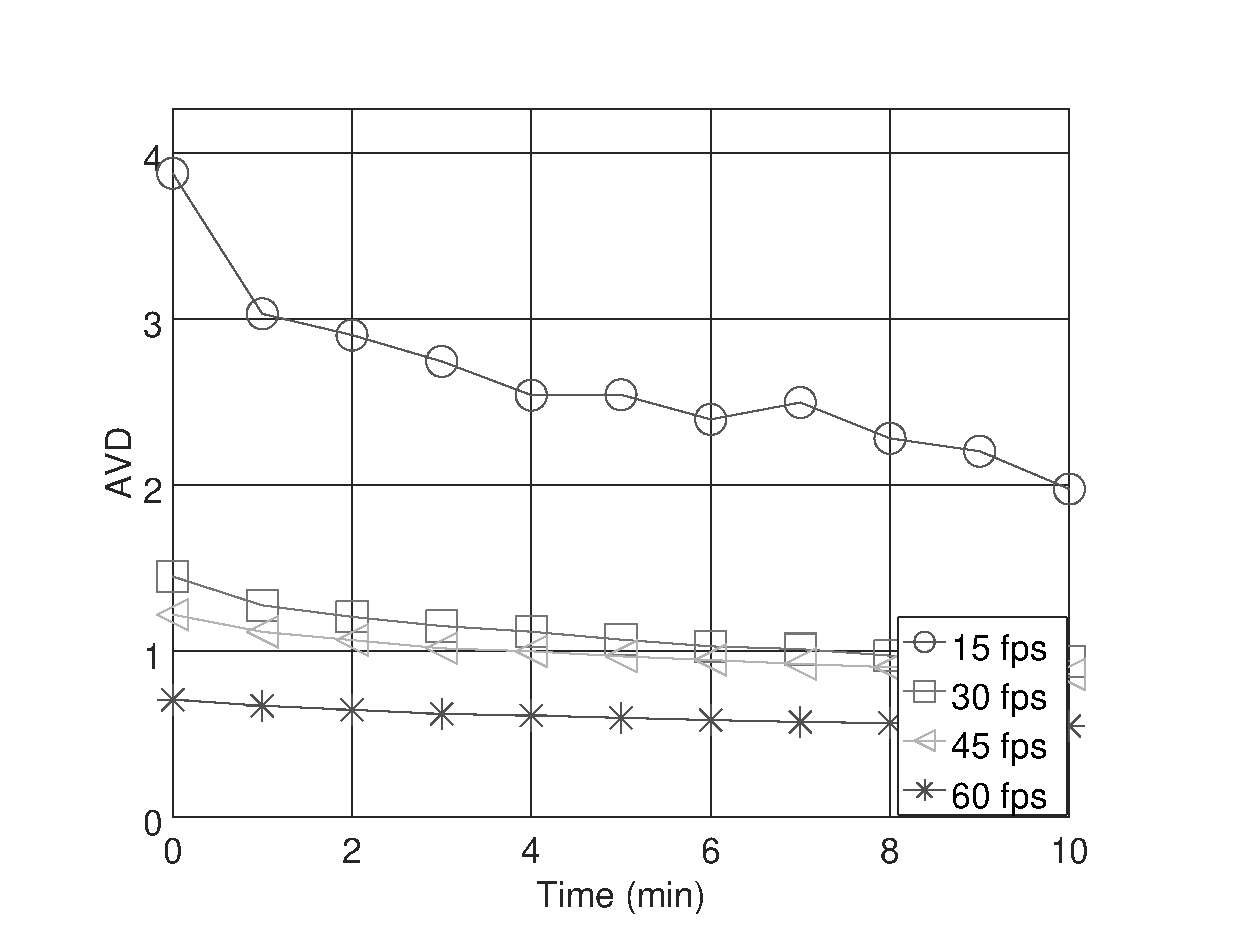
\includegraphics[width=\textwidth]{FPS_f11_rawAVD.eps}
        \label{fig:avdraw}
    \end{subfigure}
    ~ %add desired spacing between images, e. g. ~, \quad, \qquad, \hfill etc. 
      %(or a blank line to force the subfigure onto a new line)
    \begin{subfigure}{0.48\textwidth}
        \caption{Normalized $AVD$ index value.}
        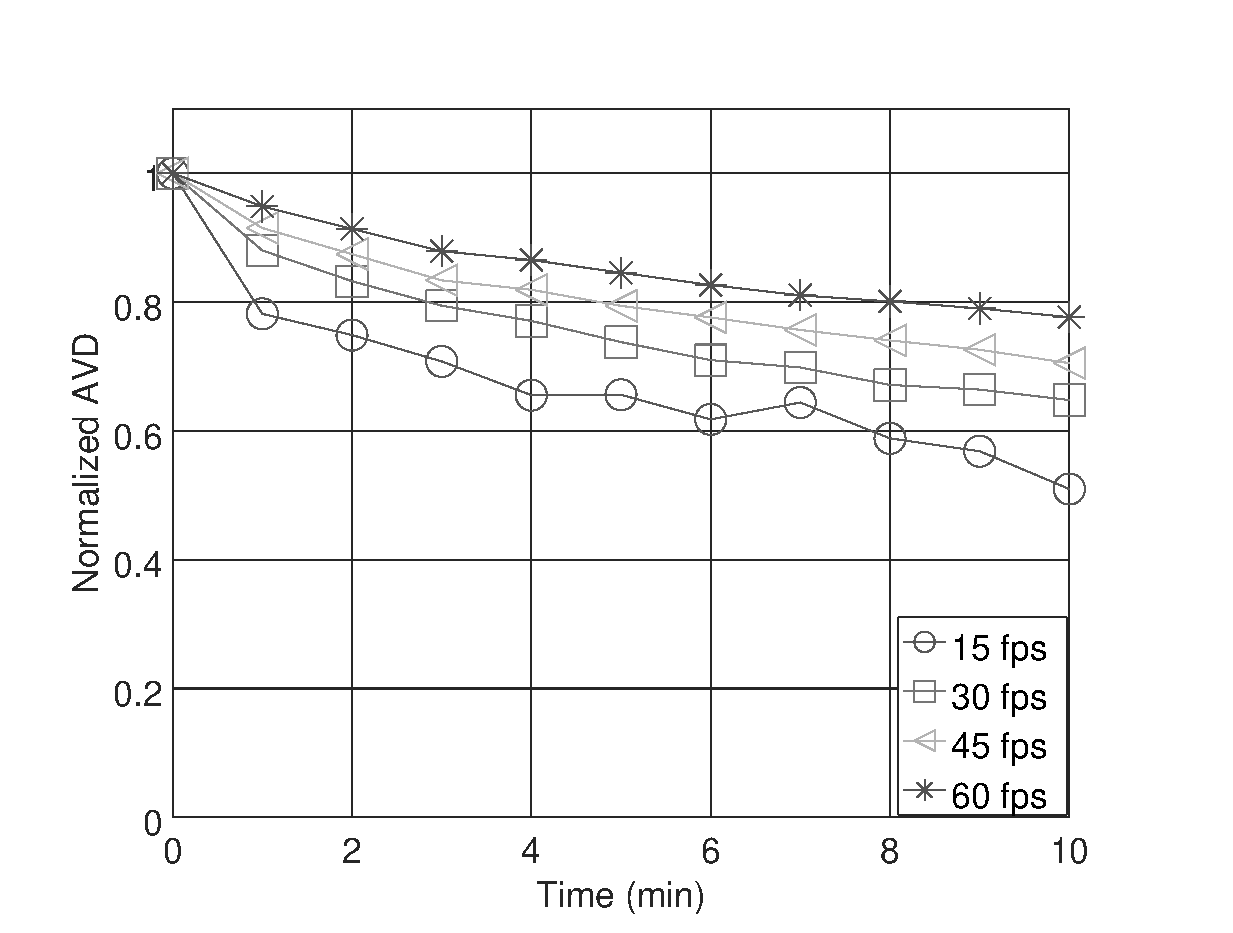
\includegraphics[width=\textwidth]{FPS_f11_norm1AVD.eps}
        \label{fig:avdnorm}
    \end{subfigure}
    \caption{$AVD$ index anaysis.}\label{fig:AVDtest1}
\end{figure}
The Figure \ref{fig:avdraw} shows the $AVD(t)$ index, in each time $t$, 
to 4 sampling frequencies, showing a different behavior across time in each sampling frequency,
so that, the value of the index in all  the curve decreases in proportion with 
the grow of sampling frequency. By other side,
the Figure \ref{fig:avdnorm} shows a normalized version of $AVD(t)$ index, 
so that the maximum value of curves have an unit value; thus,
It is easy to see that the maximum excursion of the curve is greater when decrease
the sampling frequency. Remembering that this index use information in a frequency
band between $F_s/4$ until $F_s/2$ Hz, as seen in Section \ref{sec:avd}.

%%%%%%%%%%%%%%%%%%%%%%%%%%%%%%%%%%%%%%%%%%%%%%%%%%%%%%%%%%%%%%%%%%%%%%%%%%%%%%%%
The Figure \ref{fig:STDtest1} analyze the $STD(t)$ index in the test showed in the 
Section \ref{subsec:test1}.
\begin{figure}[ht!]
    \centering
    \begin{subfigure}{0.48\textwidth}
        \caption{$STD$ index value.}
        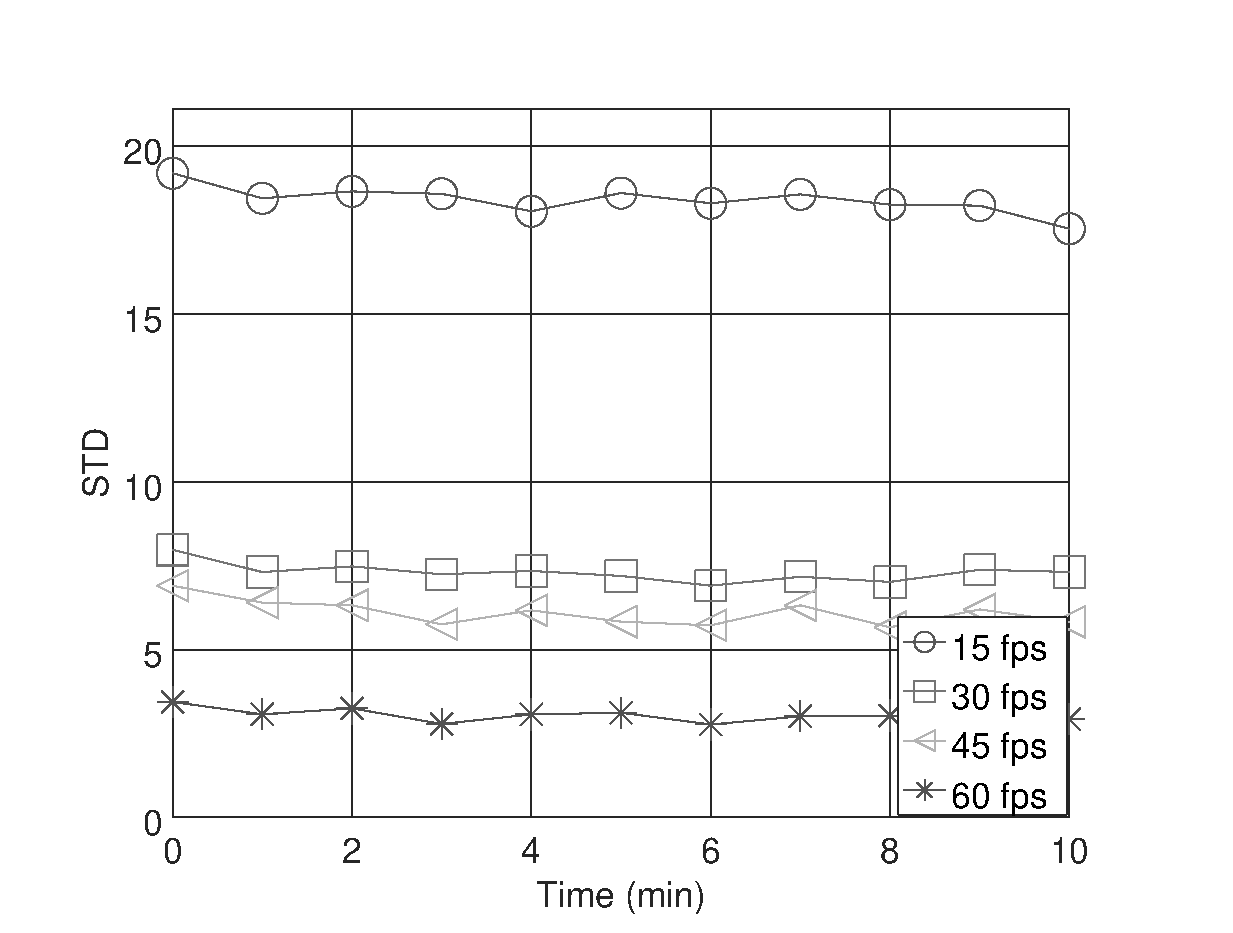
\includegraphics[width=\textwidth]{FPS_f11_rawSTD.eps}
        \label{fig:stdraw}
    \end{subfigure}
    ~ %add desired spacing between images, e. g. ~, \quad, \qquad, \hfill etc. 
      %(or a blank line to force the subfigure onto a new line)
    \begin{subfigure}{0.48\textwidth}
        \caption{Normalized $STD$ index value.}
        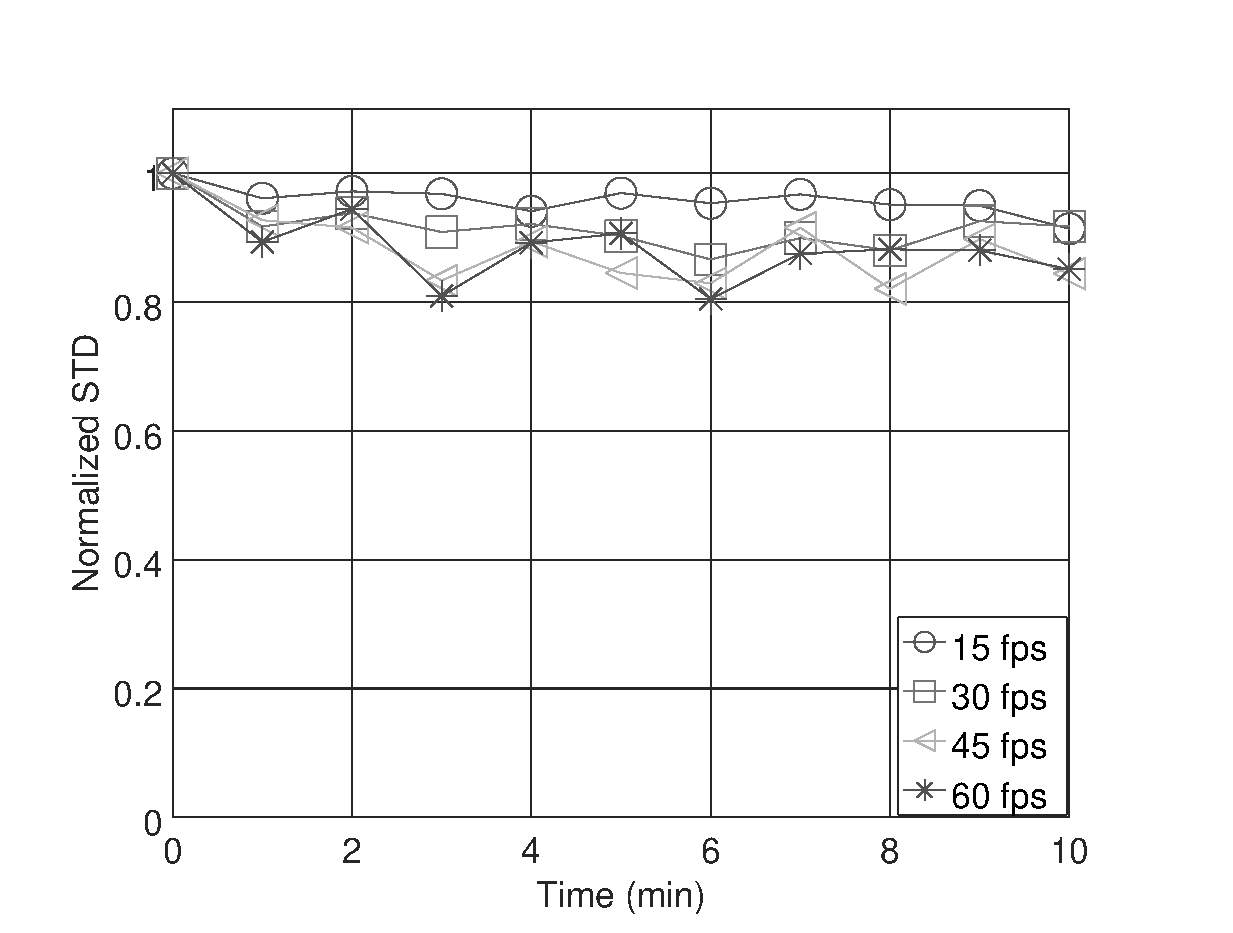
\includegraphics[width=\textwidth]{FPS_f11_norm1STD.eps}
        \label{fig:stdnorm}
    \end{subfigure}
    \caption{$STD$ index anaysis.}\label{fig:STDtest1}
\end{figure}
The Figure \ref{fig:stdraw} shows the  behavior of $STD(t)$ index, in each time $t$, 
to 4 different sampling frequencies. Remembering that this index uses information in a frequency
band between $0$ until $F_s/2$ Hz, as seen in Section \ref{sec:std}.
This index shows a different behavior across time to each sampling frequency,
so that, the value of the index in each time of curve decreases in proportion with 
the grow of sampling frequency. By other side,
the Figure \ref{fig:stdnorm} shows a normalized version of $STD(t)$ index;
being the unit, the maximum value of curves; thus,
It is easy to see that exist a small difference between the maximum excursion 
of the curves with different sampling frequency; even so, It is possible to observe
a decrease of the maximum excursion in the curve with the grow of the sampling frequency.


%%%%%%%%%%%%%%%%%%%%%%%%%%%%%%%%%%%%%%%%%%%%%%%%%%%%%%%%%%%%%%%%%%%%%%%%%%%%%%%%
The Figure \ref{fig:STDFtest1}, analyze the $STDF(t)$ index, in the test showed in the 
Section \ref{subsec:test1}.
\begin{figure}[ht!]
    \centering
    \begin{subfigure}{0.48\textwidth}
        \caption{$STDF$ index value.}
        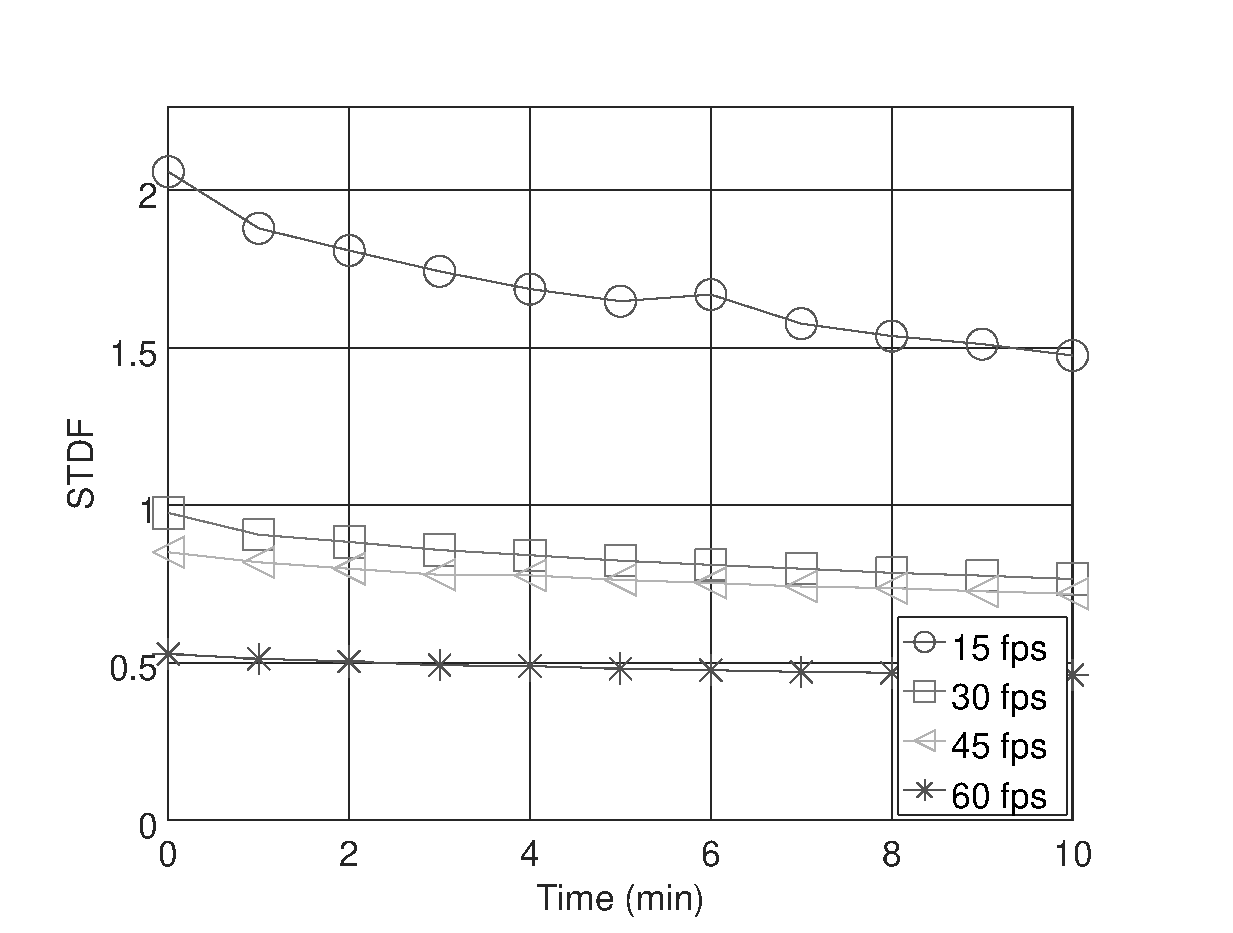
\includegraphics[width=\textwidth]{FPS_f11_rawSTDF.eps}
        \label{fig:stdfraw}
    \end{subfigure}
    ~ %add desired spacing between images, e. g. ~, \quad, \qquad, \hfill etc. 
      %(or a blank line to force the subfigure onto a new line)
    \begin{subfigure}{0.48\textwidth}
        \caption{Normalized $STDF$ index value.}
        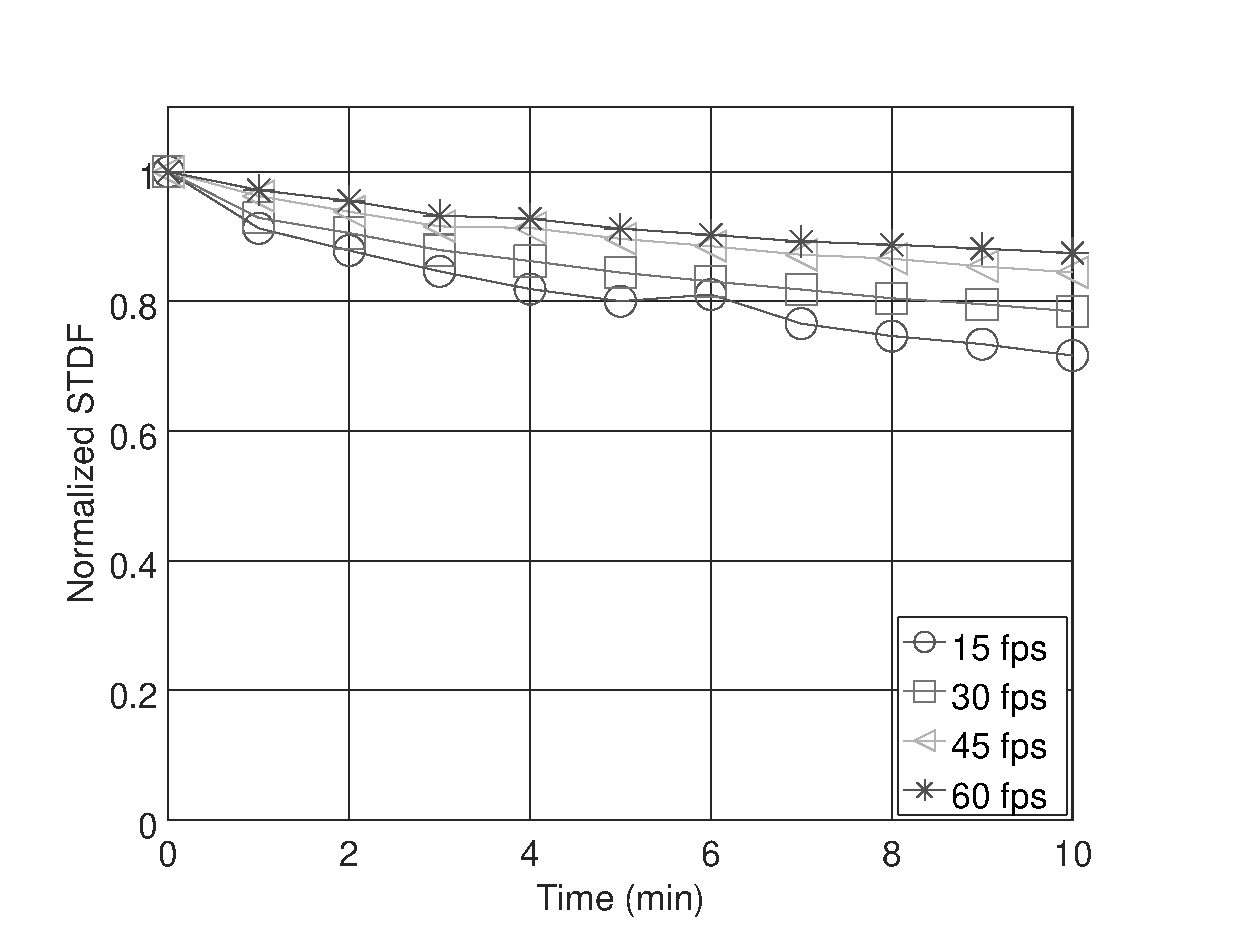
\includegraphics[width=\textwidth]{FPS_f11_norm1STDF.eps}
        \label{fig:stdfnorm}
    \end{subfigure}
    \caption{$STDF$ index anaysis.}\label{fig:STDFtest1}
\end{figure}
The Figure \ref{fig:stdfraw} shows the behavior $STDF(t)$ index, in each time $t$, 
to 4 different sampling frequencies. Remembering that this index uses filtered 
information of datapack, so that your frequency
band is between $F_s/4$ and $F_s/2$ Hz, of similar way of $AVD(t)$ index but with
different order filter, as seen in Section \ref{sec:stdf}.
This index shows monotone decreasing behavior in time, where we observe 
a different behavior across time to each different sampling frequency;
so that, the value of the index in each time of curve decreases in proportion with 
the grow of sampling frequency. By other side,
the Figure \ref{fig:stdfnorm} shows a normalized version of $STDF(t)$ index;
being the unit, the maximum value of curves; thus,
It is easy to see that exist a considerable difference between the maximum excursion 
of the curves with the use of sampling frequency; so, It is possible to observe a 
grow of the maximum excursion with the grow of the sampling frequency.

%%%%%%%%%%%%%%%%%%%%%%%%%%%%%%%%%%%%%%%%%%%%%%%%%%%%%%%%%%%%%%%%%%%%%%%%%%%%%%%%
\subsection{Result of test 2}
\label{subsec:resulttest2}

This test shows the analyze result of a corn seed  with 3 days of germination,
with the sampling frequencies: $15$, $30$, $45$ and $60$Hz.

%%%%%%%%%%%%%%%%%%%%%%%%%%%%%%%%%%%%%%%%%%%%%%%%%%%%%%%%%%%%%%%%%%%%%%%%%%%%%%%%
The Figure \ref{fig:MEANtest2} shows the $MEAN(t)$ index,
in the test described in the Section \ref{subsec:test2};
\begin{figure}[ht!]
    \centering
    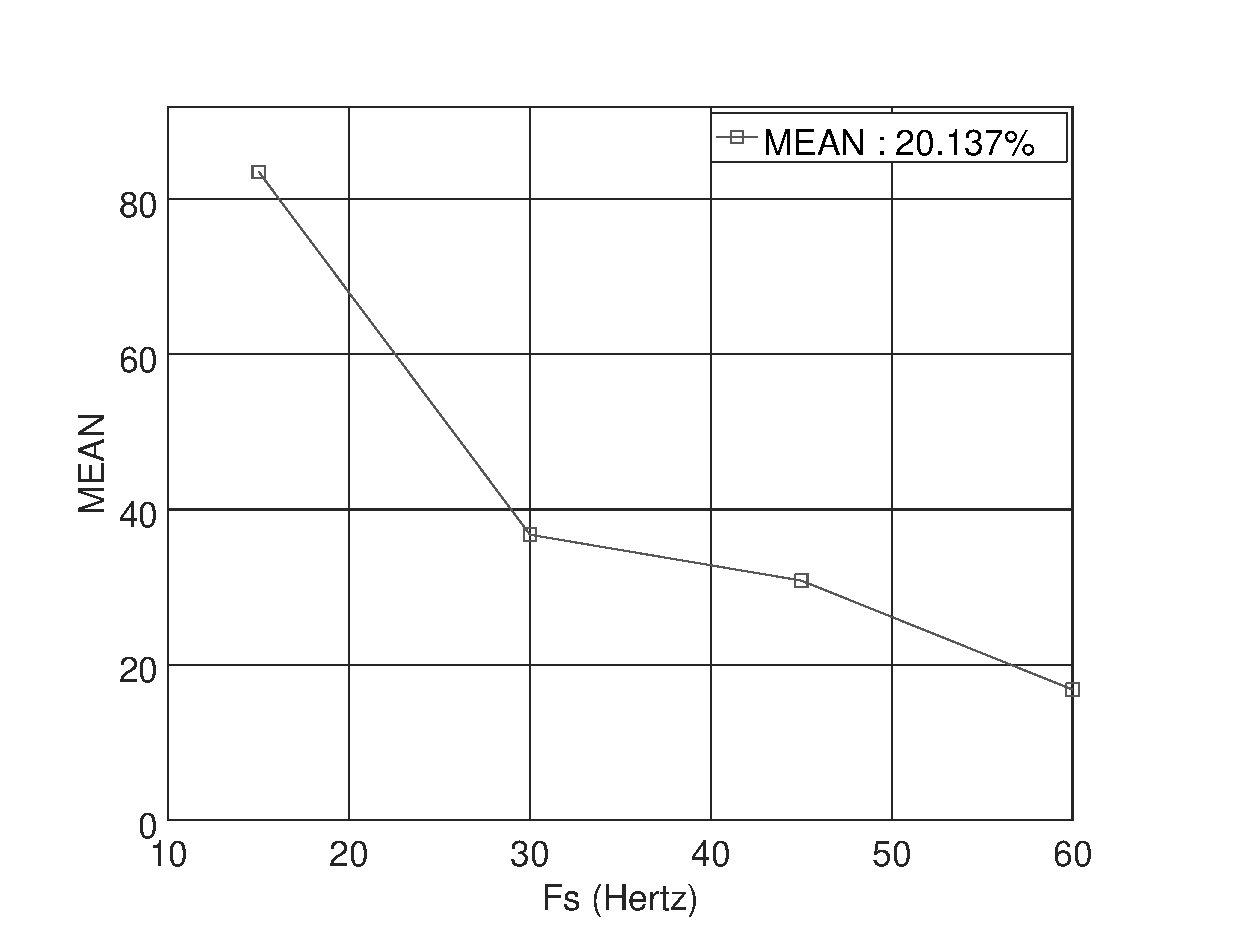
\includegraphics[width=0.5\textwidth]{FPS_Semilla_3_3diasALLMEAN.eps}
    \caption{$MEAN$ index value in the germinated corn seed.}\label{fig:MEANtest2}
\end{figure}
The figure shows as the index decrease your value, 
with the increment of sampling frequency in the datapack,
so that between $15$ Hz until $60$ Hz, the index value reaches the $20.137\%$ of your value.


%%%%%%%%%%%%%%%%%%%%%%%%%%%%%%%%%%%%%%%%%%%%%%%%%%%%%%%%%%%%%%%%%%%%%%%%%%%%%%%%
The Figure \ref{fig:INDEXtest2} shows the $AVD(t)$, $STD(t)$ and $STDF(t)$ indexes,
in the test described in the Section \ref{subsec:test2};
\begin{figure}[ht!]
    \centering
    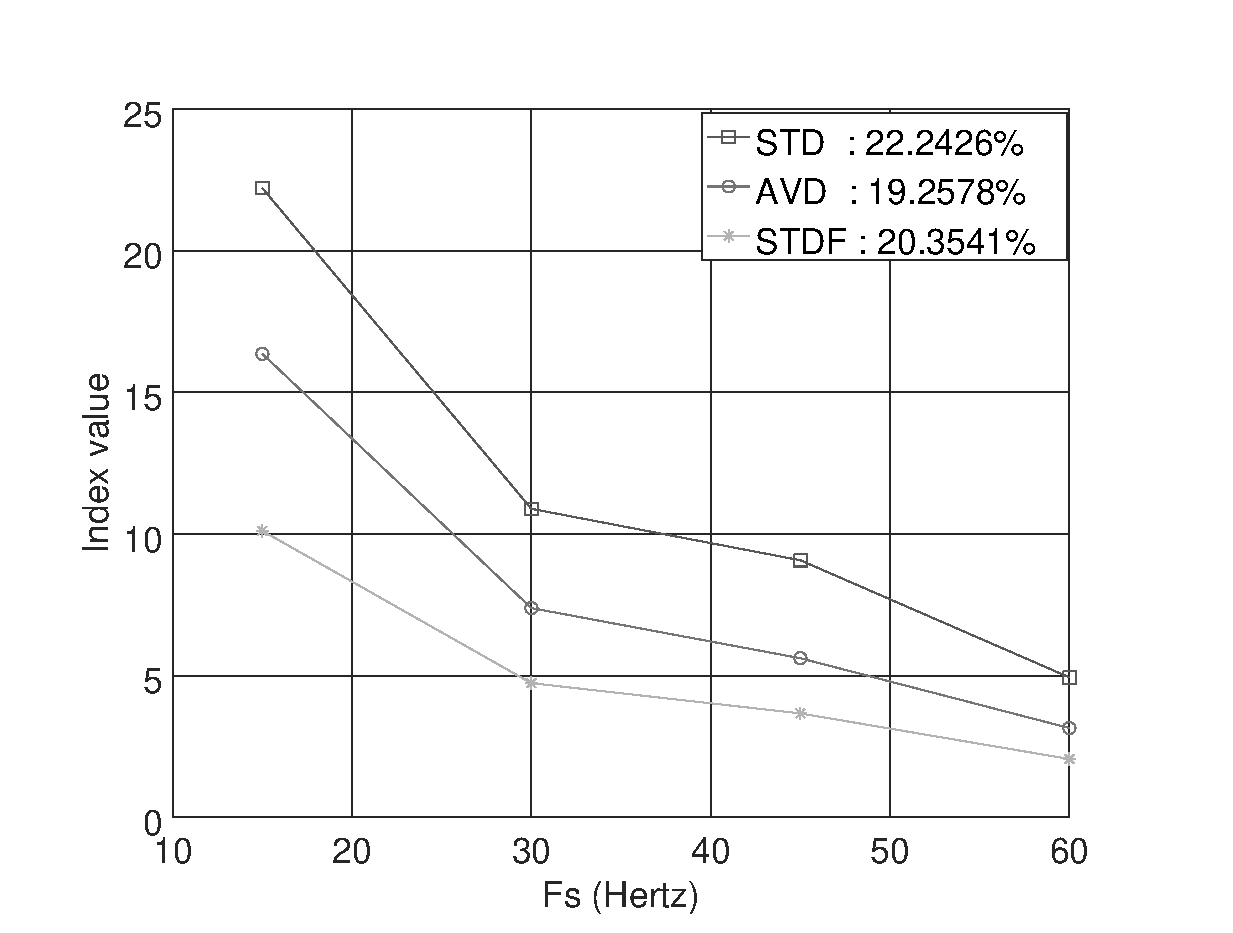
\includegraphics[width=0.5\textwidth]{FPS_Semilla_3_3diasALL.eps}
    \caption{$AVD(t)$, $STD(t)$ and $STDF(t)$ indexes values in the germinated corn seed.}\label{fig:INDEXtest2}
\end{figure}
The similar way that in the Figure \ref{fig:MEANtest2},
the index decrease your value with the grow of $F_s$,
so that the indexes, 
$AVD(t)$, $STD(t)$ and $STDF(t)$, 
reaches the $22.2426\%$, $19.2578\%$ and $20.3541\%$ of your values, 
respectively.


\subsection{Result of test 3}
\label{subsec:resulttest3}
The Table \ref{table:2} shows the result of calculating the $STDB$ image
in different frequency bands over a package $P$, see Sec. \ref{subsec:test3}, 
The package represents  a corn seed as in the Section \ref{subsec:data2};
where, we have packages sampled with the frequencies: $15$, $30$, $45$ and $60$ Hz, as
can be seen in the first column of table.

%~\\
\begin{table}[h!]
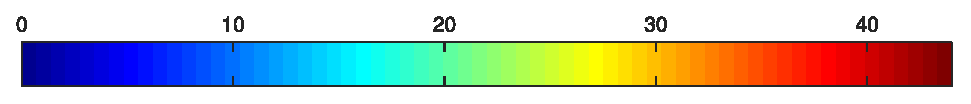
\includegraphics[width=\textwidth]{colorbar.eps}
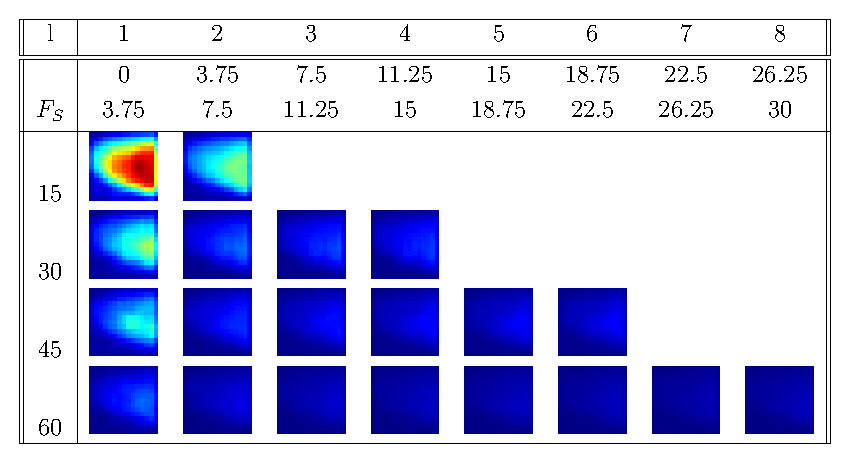
\includegraphics[width=\textwidth]{freq1.eps}
\caption{frequency band analysis}
\label{table:2}
\end{table}
In the other columns we can see the results of until $8$ frequency bands of package $P$,
these bands are represented in the first line of table, were $l$ indicates the position of frequency band
in crescent order relative to the frequency components. Thus, we have 
these frequency bands limited on: $0$, $3.75$, $7.5$, $11.25$, $15$, $18.75$, $22.5$, $26.25$ and $30$Hz.
So that, the package sampled in $15$hz was divided in $L=2$ frequency bands, 
in $30$hz was divided in $L=4$ frequency bands, 
in $45$hz was divided in $L=6$ frequency bands and finally
in $60$hz was divided in $L=8$ frequency bands.

The matrices $STDB$ are represented using a color palette, 
that goes from dark blue to dark red color, representing of ascendant way the values
in each pixel in all matrices. It is evident how the index values decreases with
the increment of frequency sampling $F_s$ in each one of 8 frequency bands, 
the index values also decrease with the increment of the position of frequency band,
being the best analysis case, 
in the sense of differentiating better places of lower and higher index, 
to a frequency sampling of $15$ hz and a frequency band between $0$ Hz and $3.75$ Hz. 




%%%%%%%%%%%%%%%%%%%%%%%%%%%%%%%%%%%%%%%%%%%%%%%%%%%%%%%%%%%%%%%%%%%%%%%%%%%%%%%%
%%%%%%%%%%%%%%%%%%%%%%%%%%%%%%%%%%%%%%%%%%%%%%%%%%%%%%%%%%%%%%%%%%%%%%%%%%%%%%%%
%%%%%%%%%%%%%%%%%%%%%%%%%%%%%%%%%%%%%%%%%%%%%%%%%%%%%%%%%%%%%%%%%%%%%%%%%%%%%%%%
%%%%%%%%%%%%%%%%%%%%%%%%%%%%%%%%%%%%%%%%%%%%%%%%%%%%%%%%%%%%%%%%%%%%%%%%%%%%%%%%
\section{Analysis results} 
\label{sec:analysisresults}


In the results seen in Section \ref{sec:numericalresults},
we can observe in the Figure \ref{fig:MEANtest1} and \ref{fig:MEANtest2}, 
that the indexes show a relation between the value of curve and the sampling frequency of datapack. 
How is known \cite{Nothdurft:05}, the temporal speckle mean index is related to 
the observed illumination level in the surface of study material and correspond to zero frequency of the signal (datapack).
Thus, we can conclude that the level of illumination, perceived by the camera, 
decrease with the increment of sampling frequency. 
This is because that the exposition time is modified with the alteration of sampling frequency, 
see Section \ref{subsec:expositiontime}, 
so that less lighting is used to take the picture and consequently the 
temporal speckle mean index decrease in  your value.
In this sense, It is important have careful in to choose a sampling frequency
that give us an index value superior to noise level of test or the quantization level of the camera.


The modification of exposition time also affect  and limit other indexes,
remember that we have a quantization level between $0$ and $255$ in the camera. 
We can see this interference in the Figures \ref{fig:AVDtest1}, \ref{fig:STDtest1}, \ref{fig:STDFtest1} and \ref{fig:INDEXtest2}, 
where the $AVD(t)$, $STD(t)$ and $STDF(t)$ indexes decrease your values in concordance with the decrease of exposition time.
Other way in that  the sampling frequency affect the values of indexes,
It is that, it limits the frequency band of analyzed signal; for example,
a sampling frequency $F_s$, by the Nyquist theorem \cite{Nyquist,Shannon}, 
causes that the frequency band of analyzed signal (datapack)  will be between $0 Hz$ and $F_s/2~Hz$.
Thus, in this context we have an index as $STD(t)$ that uses information between $\langle \left. 0, F_s/2 \right ] Hz$, 
and be other side we have indexes as the $AVD(t)$ and the $STDF(t)$ index, that use information of half frequency band, 
this is between $\left [ F_s/4, F_s/2 \right ] Hz$.
In the comparison between $STD(t)$ vs  $\{$ $STDF(t)$ and $AVD(t)$ $\}$, 
we can see how the use of half, of entire frequency band, causes the decrease in the values of the curves, 
but give us considerably good values in the maximum excursion of the curve. By other side,
in the case of ink drying process, the use of complete frequency band, 
It returns low values of maximum excursion in the curves. 
The importance of excursion in this test,
 It is due the necessity of to have significant differences en the values of two states,
when the sample start or end the ink drying process.

It is necessary to highlight the importance of to choose the least value of sampling frequency $F_s$;
so that, 
the frequency band of signal contain the frequency components with the information that you want to analyze;
so that, the values of indexes have the greatest values and consequently a good excursion, 
when compared with an inert part of sample; 
By example, in the Table. \ref{table:2} is analyzed a corn seed, 
we can see as the major values of indexes are obtained to a $F_s=15$ Hz, 
analyzing frequency component between $0$ hz and $7.5$ Hz. At this point,
an additionally result is evident, when we ask ourselves, 
What is the best frequency band? where according with the test, we see that for
all frequency bands, 
the best frequency band, to the case of corn seed, is the one with the components with less frequency.
 

%%%%%%%%%%%%%%%%%%%%%%%%%%%%%%%%%%%%%%%%%%%%%%%%%%%%%%%%%%%%%%%%%%%%%%%%%%%%%%%%
%%%%%%%%%%%%%%%%%%%%%%%%%%%%%%%%%%%%%%%%%%%%%%%%%%%%%%%%%%%%%%%%%%%%%%%%%%%%%%%%
%%%%%%%%%%%%%%%%%%%%%%%%%%%%%%%%%%%%%%%%%%%%%%%%%%%%%%%%%%%%%%%%%%%%%%%%%%%%%%%%
%%%%%%%%%%%%%%%%%%%%%%%%%%%%%%%%%%%%%%%%%%%%%%%%%%%%%%%%%%%%%%%%%%%%%%%%%%%%%%%%
\section{Conclusion} 

In this work were presented comparisons of behavior of three dynamic laser speckle indexes
subject to different values of sampling frequency, thus we concluded that:
It is important to know to choose an appropriate sampling frequency, 
being recommendable to use the minimal sampling frequency possible to get an acceptable maximum excursion,
so that the phenomenon under study to be in the analyzed frequency band.
Finally, 
we show that the digitization  of speckle signal imply a restriction of frequency 
band of signal and consequently this affect the result of an speckle analysis.


%%%%%%%%%%%%%%%%%%%%%%%%%%%%%%%%%%%%%%%%%%%%%%%%%%%%%%%%%%%%%%%%%%%%%%%%%%%%%%%%
%%%%%%%%%%%%%%%%%%%%%%%%%%%%%%%%%%%%%%%%%%%%%%%%%%%%%%%%%%%%%%%%%%%%%%%%%%%%%%%%
%%%%%%%%%%%%%%%%%%%%%%%%%%%%%%%%%%%%%%%%%%%%%%%%%%%%%%%%%%%%%%%%%%%%%%%%%%%%%%%%
%%%%%%%%%%%%%%%%%%%%%%%%%%%%%%%%%%%%%%%%%%%%%%%%%%%%%%%%%%%%%%%%%%%%%%%%%%%%%%%%
\section{Acknowledgment}
We wish to acknowledge the partial financial support for this study provided by the $CAPES$ 
scholarship
$PNPD$ Program, $FAPEMIG$ and $CNPQ$.


%%%%%%%%%%%%%%%%%%%%%%%%%%%%%%%%%%%%%%%%%%%%%%%%%%%%%%%%%%%%%%%%%%%%%%%%%%%%%%%%
%%%%%%%%%%%%%%%%%%%%%%%%%%%%%%%%%%%%%%%%%%%%%%%%%%%%%%%%%%%%%%%%%%%%%%%%%%%%%%%%
%%%%%%%%%%%%%%%%%%%%%%%%%%%%%%%%%%%%%%%%%%%%%%%%%%%%%%%%%%%%%%%%%%%%%%%%%%%%%%%%
%%%%%%%%%%%%%%%%%%%%%%%%%%%%%%%%%%%%%%%%%%%%%%%%%%%%%%%%%%%%%%%%%%%%%%%%%%%%%%%%
\section{Bibliography}
\bibliography{report}   %>>>> bibliography data in report.bib
\bibliographystyle{spiebib}   %>>>> makes bibtex use spiebib.bst


\end{document} 


